\documentclass[border=10pt]{standalone}
\usepackage{pgfplots}
\pgfplotsset{compat=1.18}
\begin{document}
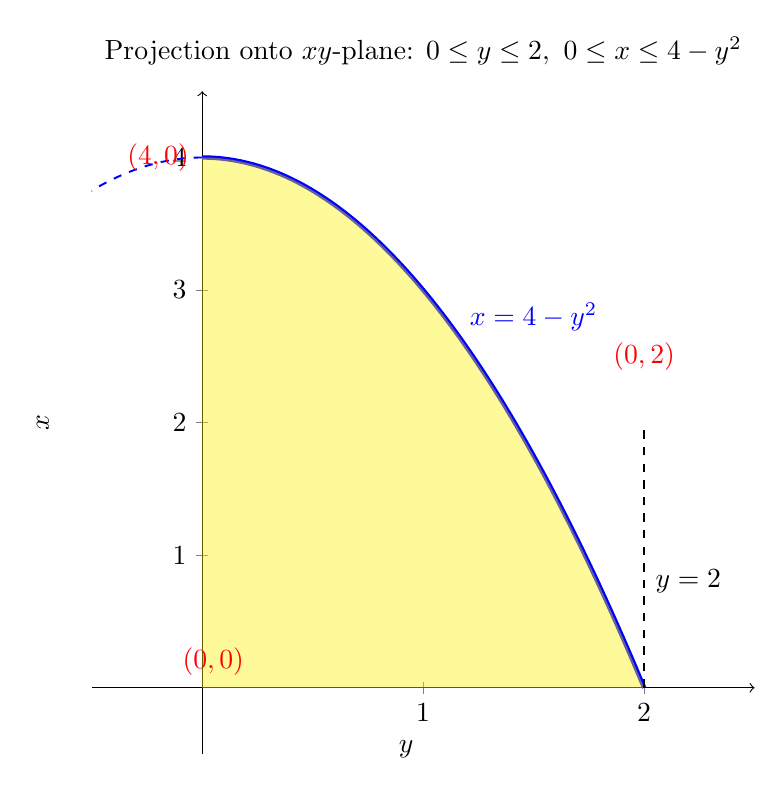
\begin{tikzpicture}
\begin{axis}[
    title={Projection onto $xy$-plane: $0\le y\le 2,\ 0\le x\le 4-y^2$},
    xlabel={$y$}, ylabel={$x$},
    xmin=-0.5, xmax=2.5, ymin=-0.5, ymax=4.5,
    xtick={0,1,2}, ytick={0,1,2,3,4},
    width=10cm, height=10cm,
    axis lines=middle, axis line style={->},
    xlabel style={at={(axis description cs:0.5,-0.02)}},
    ylabel style={at={(axis description cs:-0.05,0.5)}, rotate=90, anchor=south},
]
% Parabola
\addplot[domain=0:2, samples=80, blue, line width=1.6pt] (\x, {4-\x*\x});
\addplot[domain=-2:0, samples=80, blue, line width=0.7pt, dashed] (\x, {4-\x*\x});

% Fill the parabolic region
\addplot[domain=0:2, samples=80, fill=yellow, fill opacity=0.4, draw=none]
    (\x, {4-\x*\x}) \closedcycle;

% y=2 boundary
\addplot[black, line width=0.8pt, dashed] coordinates {(2,0) (2,2)};
% labels
\node[red] at (axis cs:2,2.5) {$(0,2)$};
\node[red] at (axis cs:-0.2,4) {$(4,0)$};
\node[red] at (axis cs:0.05,0.2) {$(0,0)$};
\node at (axis cs:2.2, 0.8) {$y=2$};
\node[blue] at (axis cs:1.5, 2.8) {$x=4-y^2$};
\end{axis}
\end{tikzpicture}
\end{document}